Inductive learning of symbolic expressions for continuous-valued time series
data is a hard task which has recently been tackled using a greedy search over 
the approximate posterior of the possible kernel compositions for
\ac{GP}s~\citep{duvenaud2013structure,lloyd2014automatic}\footnote{\url{http://www.automaticstatistician.com/}}.

With \gpmem\ we can provide a fully Bayesian treatment of this, previously unavaible,
using a stochastic grammar  (see Fig. \ref{fig:schema}).
%%%%%%%%%%%%%%%%%%%%%%%%%%%%%%%%%%%%%%%%%%%%%%%%%%%%%%%%%%%%
\begin{figure}
\centering
\usetikzlibrary{arrows, decorations.markings}
\usetikzlibrary{trees}

\tikzstyle{level 1}=[level distance=1cm, sibling distance=1.5cm]
\tikzstyle{level 2}=[level distance=1cm, sibling distance=1.1cm]

% Define styles for operators and leafs
\tikzstyle{operator} = [draw=none,circle, minimum width=1pt]
\tikzstyle{end} = [circle, minimum width=3pt,fill, inner sep=0pt]
% for double arrows a la chef
% adapt line thickness and line width, if needed

\begin{subfigure}[b]{0.49\textwidth}\centering
\begin{tikzpicture}[thick]
 \node[] (start) {};
 \node[left=-0.2cm of start] (base_kernels) {\small$\{\Kbf_{\bm{\theta}^1}^1,\cdots,\Kbf_{\bm{\theta}^m}^m\}$};
 \node[above=0.7cm of base_kernels] (theta) {\small$\bm{\theta}^* \sim P(\bm{\theta}^*)$};
\node[right=0.5cm of start] (n) {$P(n)$};
 \node[draw,rectangle, below=1cm of start, text width =6.0cm, text 
height=4.1cm,align=center] (grammar)
{};


 \node[draw,dashed,rectangle, below=-3.8cm of grammar, text width
=4.7cm,align=center] (subset) {
$\;\;\;\;\;\;\;\;\;\;\;\;$Subset SP % I can't believe that this is the simpliest way to
% get spacing right 
{\raggedright
\footnotesize$ n\; \sim P(n),\;\;\;\;\; n \leq m$ \\

\footnotesize$S \; \sim P(S = \{\Kbf_{\bm{\theta}^i}^i,\cdots,\Kbf_{\bm{\theta}^n}^n\} \mid n)$
}
};
 \node[draw,rectangle,dashed, below=0.7cm of subset, text width
=4.35cm,align=center]
(composition_procedure) {
$\;$Composition Procedure\\ % I can't believe that this is the simpliest way to
% get spacing right 
{\raggedright
\footnotesize$\bm{\Omega}\;\; \sim P(\bm{\Omega} \mid S,n)$ \\

\footnotesize$\Kbf_{\bm{\theta}} \sim P(\Kbf_{\bm{\theta}} \mid \bm{\Omega},S,n),\;\,\bm{\theta}\subseteq\bm{\theta}^*$
}
};

\node[above=0.0cm of subset]{\centering \bf Stochastic Grammar}; 

 \node[draw,rectangle,below=1cm of grammar] (gpmem) {\texttt{gpmem}};

 \node[draw,rectangle,below=1cm of gpmem] (f) {Data Generation};
\node[left of=f,xshift=-1.5cm] (x) {$\mathbf{t}$};
\node[right of=f,xshift=1.5cm] (y) {$\mathbf{f}$};

 \node[below=0.1cm  of grammar,xshift=0.5cm] (k)
{\small$\Kbf_{\bm{\theta}}$};


\node[below=0.1cm  of gpmem,xshift=0.6cm] (gp) {
\small$f_{emu}$};

% 1st pass: draw arrows
  \draw[thick,->] (base_kernels) -- (grammar);
  \draw[thick,->] (n) -- (grammar);
  \draw[thick,->] (theta) -- (base_kernels);
  \draw[thick,->] (grammar) -- (gpmem);
  \draw[thick,->] (gpmem) -- (f);
 \draw[thick,->] (x) -- (f);
 \draw[thick,->] (f) -- (y);
 \draw[thick,dashed,->] (subset) -- node[right]{\footnotesize $\;S$} (composition_procedure);
  % Note: If you have no branches, the 2nd pass is not needed
\end{tikzpicture}\vspace{2mm}
\caption{} 
\end{subfigure}
\begin{subfigure}[b]{0.49\textwidth}\centering
\begin{tikzpicture}[grow=right, sloped]
\node[operator] {\small $+$}
    child {
        node[operator] {\small $+$}        
            child {
               node[operator] {\small $\times$}        
        child {
                node[operator, label=right:
                    {$\cdots$}] {}
                edge from parent
                node[above] {}
                node[below]  {}
            }
            child {
                node[end, label=right:
                    {SE$_{\theta^4}$}] {}
                edge from parent
                node[above] {}
                node[below]  {}
            }
        edge from parent         
            node[above] {}
            node[below]  {}
            }
            child {
                node[end, label=right:
                    {WN$_{\theta^3}$}] {}
                edge from parent
                node[above] {}
                node[below]  {}
            }
            edge from parent 
            node[above] {}
            node[below]  {}
    }
    child {
        node[operator] {\small $\times$}        
        child {
                node[end, label=right:
                    {PER$_{\theta^2}$}] {}
                edge from parent
                node[above] {}
                node[below]  {}
            }
            child {
                node[end, label=right:
                    {LIN$_{\theta^1}$}] {}
                edge from parent
                node[above] {}
                node[below]  {}
            }
        edge from parent         
            node[above] {}
            node[below]  {}
    };
\node[xshift=-0.7cm] (K) {$\mathbf{K}_{\bm{\theta}}=$}; 
 \node[xshift=2.6cm,below =2.4cm of K] (Keq) {$\mathbf{K}_{\bm{\theta}}=\text{LIN}_{\theta^1} \times \text{PER}_{\theta^2}+\text{WN}_{\theta^3} + \text{SE}_{\theta^4} \times ( \cdots )$};
\end{tikzpicture}
\caption{} 
\end{subfigure}

\begin{subfigure}[b]{0.99\textwidth}\centering
\begin{tabular}{cccc}
\multicolumn{4}{c}{\bf Base Components} \rule{0pt}{3ex} \\ 
\small LIN: Linearity &\small PER: Periodicity &\small SE: Smoothness &\small WN: White Noise \rule{0pt}{2ex} \\
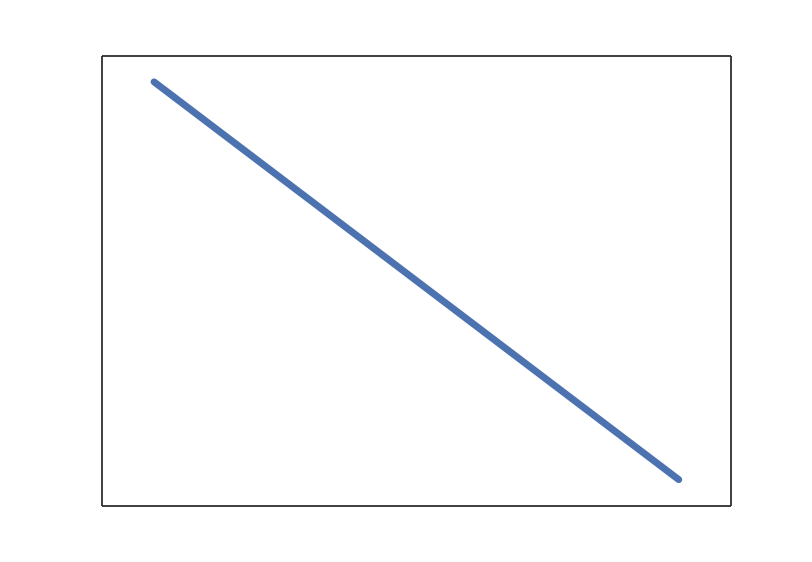
\includegraphics[height=2cm]{figs/kernel/kernelLIN.png} & 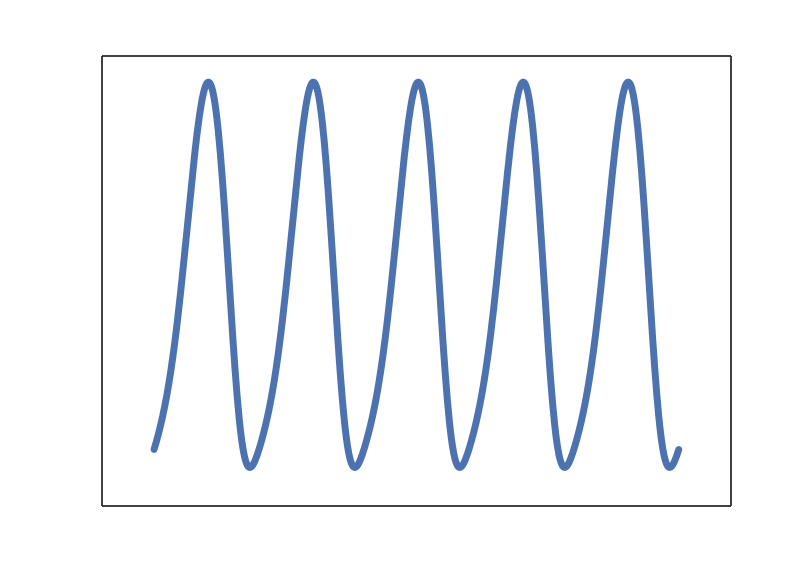
\includegraphics[height=2cm]{figs/kernel/kernelPER.png} & 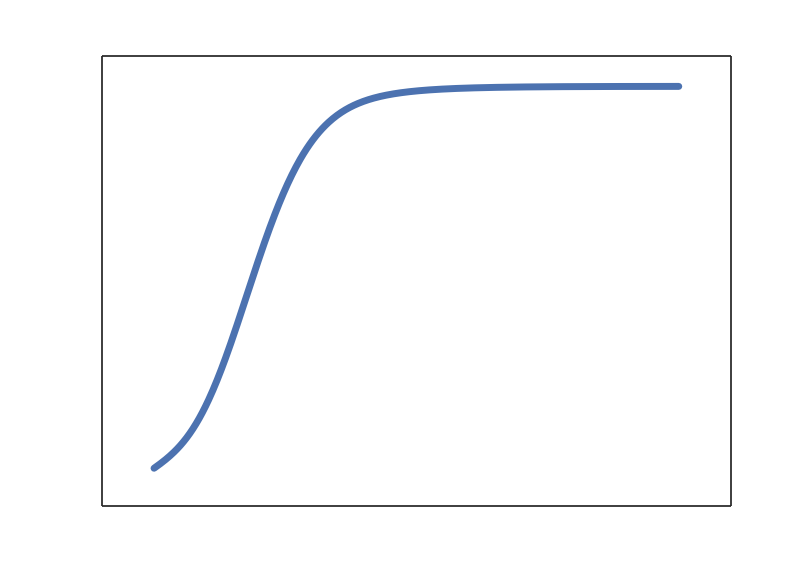
\includegraphics[height=2cm]{figs/kernel/kernelSE.png} & 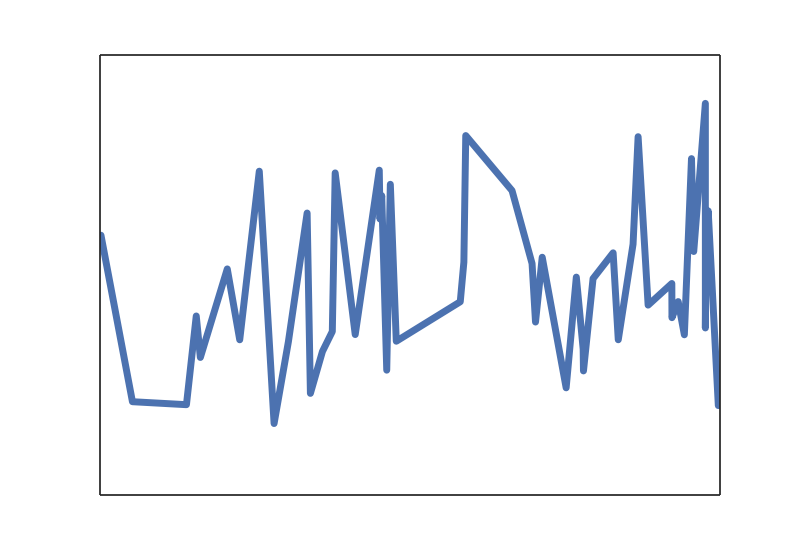
\includegraphics[height=2cm]{figs/kernel/kernelWN.png}\\
\end{tabular}
\begin{tabular}{cccc}
\multicolumn{4}{c}{\bf Composite Structure} \rule{0pt}{0ex}  \\ 
\small LIN + PER: &\small LIN $\times$ PER: &\small SE $\times$ PER: &\small LIN $\times$ LIN: \rule{0pt}{2ex} \\
\small Periodicity with Trend &\small Growing Amplitude &\small Local Periodicity&\small Quadratic \rule{0pt}{2ex} \\
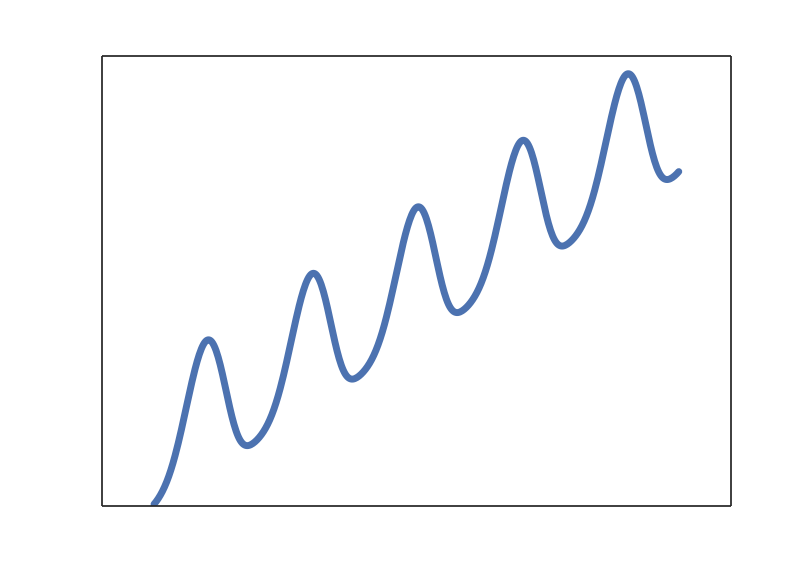
\includegraphics[height=2cm]{figs/kernel/kernelLINplusPER.png} & 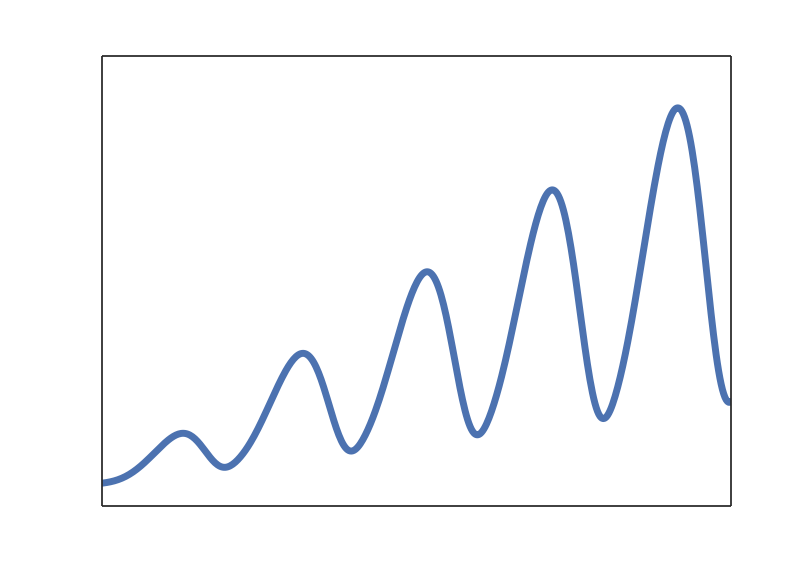
\includegraphics[height=2cm]{figs/kernel/kernelLINtimesPER.png} & 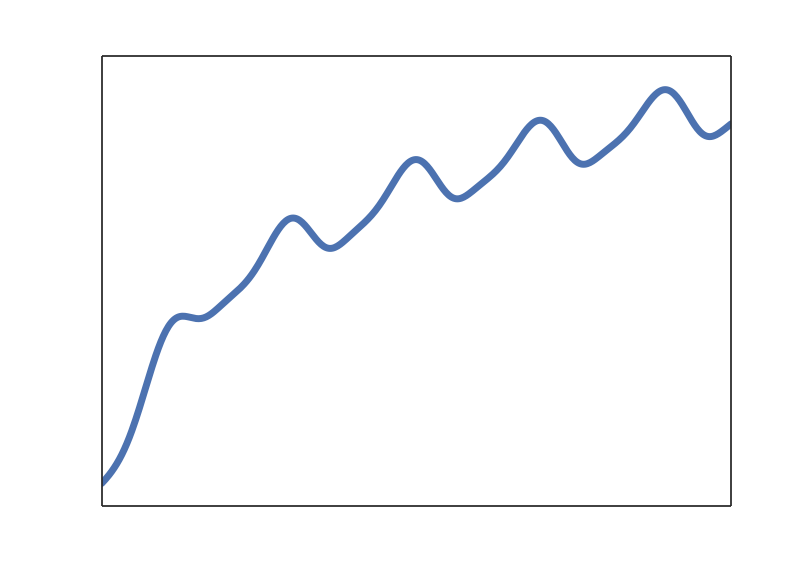
\includegraphics[height=2cm]{figs/kernel/kernelSEplusPER.png}& 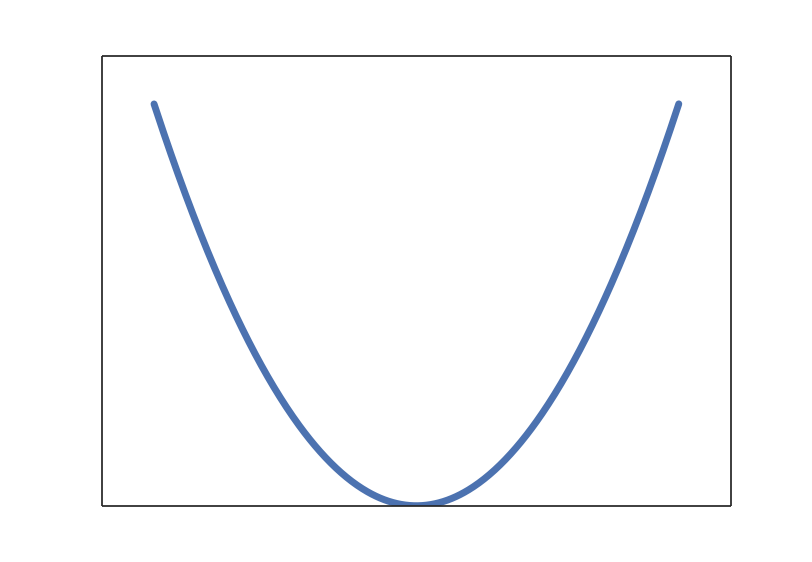
\includegraphics[height=2cm]{figs/kernel/kernelLINtimesLIN.png}\\
\end{tabular}
\caption{}
\end{subfigure}

\caption{\footnotesize (a) Bayesian GP structure learning. A set of
base kernels (BK) with priors on their hyper-parameters serves as hypothesis space
and is supplied as input to the stochastic grammar. The stochastic grammar has
two parts: (i) a sampler that selects a random set $\Sbf$  of primitive kernels from BK
and (ii) a kernel composer that combines the individual base kernels and generates
a composite kernel function
$k_{\thetabf}$. This serves as input for
\gpmem.  We observe value pairs $\xbf,\ybf$ of unstructured time series data on
the bottom of the schematic.
(b) We use $\Parse(\ktheta)$ to parse a structure. (c) kernel functions are
simplified with the $\Simplify()$-operator. The simplifed $\ktheta$ is used as input for
$\Struct()$ (d) which  interprets it symbolically.
Base kernels and compositional kernels are shown in (e) alongside their
interpretation with Struct().}\label{fig:schema}
\end{figure}
%%%%%%%%%%%%%%%%%%%%%%%%%%%%%%%%%%%%%%%%%%%%%%%%%%%%%%%%%%%%
This allows us to read an unstructured time series and automatically output a high-level,
qualitative description of it. The stochastic grammar takes a set of primitive base kernels 
    $\text{BK}=\{k_{\bm{\theta}^1}^1,\cdots,k_{\bm{\theta}^m}^m\}$

    $\thetabf^*=\{\thetabf^1,\cdots,\thetabf^m\}$ (Fig. \ref{fig:schema} (a) and (b))
We depict the input for the
stochastic grammar in Listing \ref{alg:base_kernels}.

We sample a random subset $\Sbf$ of
the set of supplied base kernels. $\Sbf$ is of size $n \leq m$. We write
%%%%%%%%%%%%%%%%%%%%%%%%%%%%%%%%%%%%%%%%%%%%%%%%%%%%%%%%%%%%
\[
\Sbf = \{k_{\bm{\theta}^i}^i,\cdots,k_{\bm{\theta}^n}^n\}
\sim P(\Sbf = \{k_{\bm{\theta}^i}^i,\cdots,k_{\bm{\theta}^n}^n\} \mid
\text{BK}) 
\]
%%%%%%%%%%%%%%%%%%%%%%%%%%%%%%%%%%%%%%%%%%%%%%%%%%%%%%%%%%%%
with
%%%%%%%%%%%%%%%%%%%%%%%%%%%%%%%%%%%%%%%%%%%%%%%%%%%%%%%%%%%%
\[
P(\Sbf = \{k_{\bm{\theta}^i}^i,\cdots,k_{\bm{\theta}^n}^n\}\mid \text{BK}) =
\frac{n!}{ \mid \Sbf = \{k_{\bm{\theta}^i}^i,\cdots,k_{\bm{\theta}^n}^n\}\mid !}.
\]
%%%%%%%%%%%%%%%%%%%%%%%%%%%%%%%%%%%%%%%%%%%%%%%%%%%%%%%%%%%%

BK is assumed to be fixed as the most general margin of our hypothesis space.
In the following, we will drop it in the notation.
The only building block that we are now missing is how to combine the sampled
base kernels into a compositional covariance function (see Fig. \ref{fig:schema}
(b)). For each interaction $i$, we
have to infer whether the data supports a local interaction or a global interaction,
chosing between one out of two algebraic operators
$\bm{\Omega}_i=\{+,\times\}$. The probability for all such decisions is given by a binomial distribution: 
\begin{equation}
P(\bm{\Omega} \mid \Sbf)= {n \choose r}  p_{+\times}^r (1 - p_{+\times})^{n-r}.
\end{equation}
We can write the marginal probability of a kernel function as 
%%%%%%%%%%%%%%%%%%%%%%%%%%%%%%%%%%%%%%%%%%%%%%%%%%%%%%%%%%%%
\begin{equation}
P(\Krv \mid \xbf,\ybf,\thetabf ) = \iint \limits_{\bm{\Omega},\Sbf}
P(\Krv \mid \xbf,\ybf,\thetabf,\bm{\Omega},\Sbf) \times P(\bm{\Omega} \mid \Sbf)\times
P(\Sbf)\; \text{\bf d}\bm{\Omega}\, \text{\bf d}\Sbf\,
\end{equation}
%%%%%%%%%%%%%%%%%%%%%%%%%%%%%%%%%%%%%%%%%%%%%%%%%%%%%%%%%%%%
with $\bm{\theta}\subseteq \bm{\theta}^*$ as implied by $\Sbf$.
For structure learning with \ac{GP} kernels, a composite kernel is
sampled from $P(\Krv)$ and fed into \gpmem. 
The emulator generated by \gpmem\ observes unstructured time series data.
Venture code for the probabilistic grammar is shown in Listing
\ref{alg:grammar}, code for inference with \gpmem\ in Listing
\ref{alg:structureVent}. 
\begin{mdframed}
\begin{minipage}{\linewidth}
\small
\belowcaptionskip=-10pt
\begin{lstlisting}[mathescape,label=alg:base_kernels,basicstyle=\selectfont\ttfamily,numbers=none,caption={Initialize
Base Kernels BK and $P(n)$},escapechar=\#]
#\linenumber{1}# // Initialize hyper-parameters
#\linenumber{2}#assume theta_1 = tag("hyper-parameters", 1, gamma(5,1));
#\linenumber{3}#assume theta_2 = tag("hyper-parameters", 2, gamma(5,1));
#\linenumber{4}#assume theta_3 = tag("hyper-parameters", 3, gamma(5,1));
#\linenumber{5}#assume theta_4 = tag("hyper-parameters", 4, gamma(5,1));
#\linenumber{6}#assume theta_5 = tag("hyper-parameters", 5, gamma(5,1));
#\linenumber{7}#assume theta_6 = tag("hyper-parameters", 6, gamma(5,1));
#\linenumber{8}#assume theta_7 = tag("hyper-parameters", 7, gamma(5,1));
#\linenumber{9}#
#\linenumber{11}# // Make kernels
#\linenumber{12}#assume lin = apply_function(make_linear, theta_1);
#\linenumber{13}#assume per = apply_function(make_periodic, theta_2, theta_3, theta_4);
#\linenumber{14}#assume se  = apply_function(make_squaredexp, theta_5, theta_6);
#\linenumber{15}#assume wn  = apply_function(make_noise, theta_7);
#\linenumber{16}#
#\linenumber{17}#// Initialize the set of primitive base kernels BK 
#\linenumber{18}#assume BK = list(lin, per, se, wn);
\end{lstlisting}
\end{minipage}
\end{mdframed}








Many equivalent covariance structures can be sampled due to covariance function algebra
and equivalent representations with different parameterization~\citep{lloyd2014automatic}.
To inspect the posterior of these equivalent structures we convert each kernel expression
into a sum of products and subsequently simplify. 
We introduce three different operators that work on kernel functions:
\begin{enumerate}
\item $\Parse(k)$, an operator that parses a covariance function (Fig.
\ref{fig:schema} (b)). 
\item $\Simplify(k)$; this operators simplifies a kernel function $k$ according
to the simplifications that we present in Appendix B and Fig.
\ref{fig:schema} (c).
\item $\Struct(k)$; interprets the structure of a covariance function (Fig.
\ref{fig:schema} (d) and Appendix C), for
example $\Struct(\klin)=\text{LIN}$; it translates the functional structure
into a symbolic expression. 
\end{enumerate}
All base kernels relevant for this work can be found in Appendix A.
\begin{mdframed}
\begin{minipage}{\linewidth}
\small
\belowcaptionskip=-10pt
\begin{lstlisting}[mathescape,label=alg:grammar,basicstyle=\selectfont\ttfamily,numbers=none,caption={
Stochastic Grammar},escapechar=\#]
#\linenumber{1}#// Select a random subset of the set possible primitive kernels (BK)
#\linenumber{2}#assume primitive_kernel_selection = tag("grammar", 0,
#\linenumber{3}#				 select_primitive_kernels(BK));
#\linenumber{4}#// Construct kernel composition with a composer procedure
#\linenumber{5}#assume kernel_composer = proc(l) {
#\linenumber{6}#  if (size(l) <= 1) {
#\linenumber{7}#    first(l)
#\linenumber{8}#  } else {
#\linenumber{9}#       if (bernoulli()) {
#\linenumber{10}#            add_funcs(first(l),  kernel_composer(rest(l)))
#\linenumber{11}#       } else {
#\linenumber{12}#            mult_funcs(first(l), kernel_composer(rest(l)))
#\linenumber{13}#    }
#\linenumber{14}#  }
#\linenumber{15}#};
#\linenumber{16}#
#\linenumber{17}#assume K = tag("grammar", 1,
	        	kernel_composer(primitive_kernel_selection));
\end{lstlisting}

\end{minipage}
\end{mdframed}

\begin{mdframed}
\begin{minipage}{\linewidth}
\small
\belowcaptionskip=-10pt
\begin{lstlisting}[mathescape,label=alg:structureVent,basicstyle=\selectfont\ttfamily,numbers=none,caption={\gpmem\
inference for structure
learning: },escapechar=\#]
#\linenumber{1}#// Apply gpmem 
#\linenumber{2}#assume (f_compute, f_emu) = gpmem(f_look_up, K);
#\linenumber{3}#// Probe all data points
#\linenumber{4}#for (n = 0; n < size(data); n++) { 
#\linenumber{5}#	predict f_compute(first(lookup(data, n)))};
#\linenumber{6}#// Perform inference
#\linenumber{7}#infer repeat(200, do(
#\linenumber{8}#	mh("grammar", one, 1),
#\linenumber{9}#	mh("hyper-parameters", one, 2)));
\end{lstlisting}

\end{minipage}
\end{mdframed}


%%%%%%%%%%%%%%%%%%%%%%%%%%%%%%%%%%%%%%%%%%%%%%%%%%%%%%%%%%%%%%%%%%%%%%%%%%%%%%%%%
%%%%%%%%%%%%%%%%%%%%%%%%%     Mauna result      %%%%%%%%%%%%%%%%%%%%%%%%%%%%%%%%%%
%%%%%%%%%%%%%%%%%%%%%%%%%%%%%%%%%%%%%%%%%%%%%%%%%%%%%%%%%%%%%%%%%%%%%%%%%%%%%%%%%
\newpage
We defined a simple space of covariance structures in a way that allows us to produce results coherent with 
work presented in Automatic Statistician~\citep{duvenaud2013structure,lloyd2014automatic}. The results are illustrated with two data sets.

\myparagraph{Mauna Loa  CO$_2$ data}
%%%%%%%%%%%%%%%%%%%%%%%%%%%%%%%%%%%%%%%%%%%%%%%%%%%%%%%%%%%%%%%%%%%%%%%%%%%%%%%%%
\begin{figure}
\centering
 \addtolength\abovedisplayskip{-1\baselineskip}%
  \addtolength\belowdisplayskip{-1\baselineskip}%
 
\begin{tikzpicture}
\node (datatitle) {\small Raw Data};
\node[below = -0.25cm of datatitle] (data) {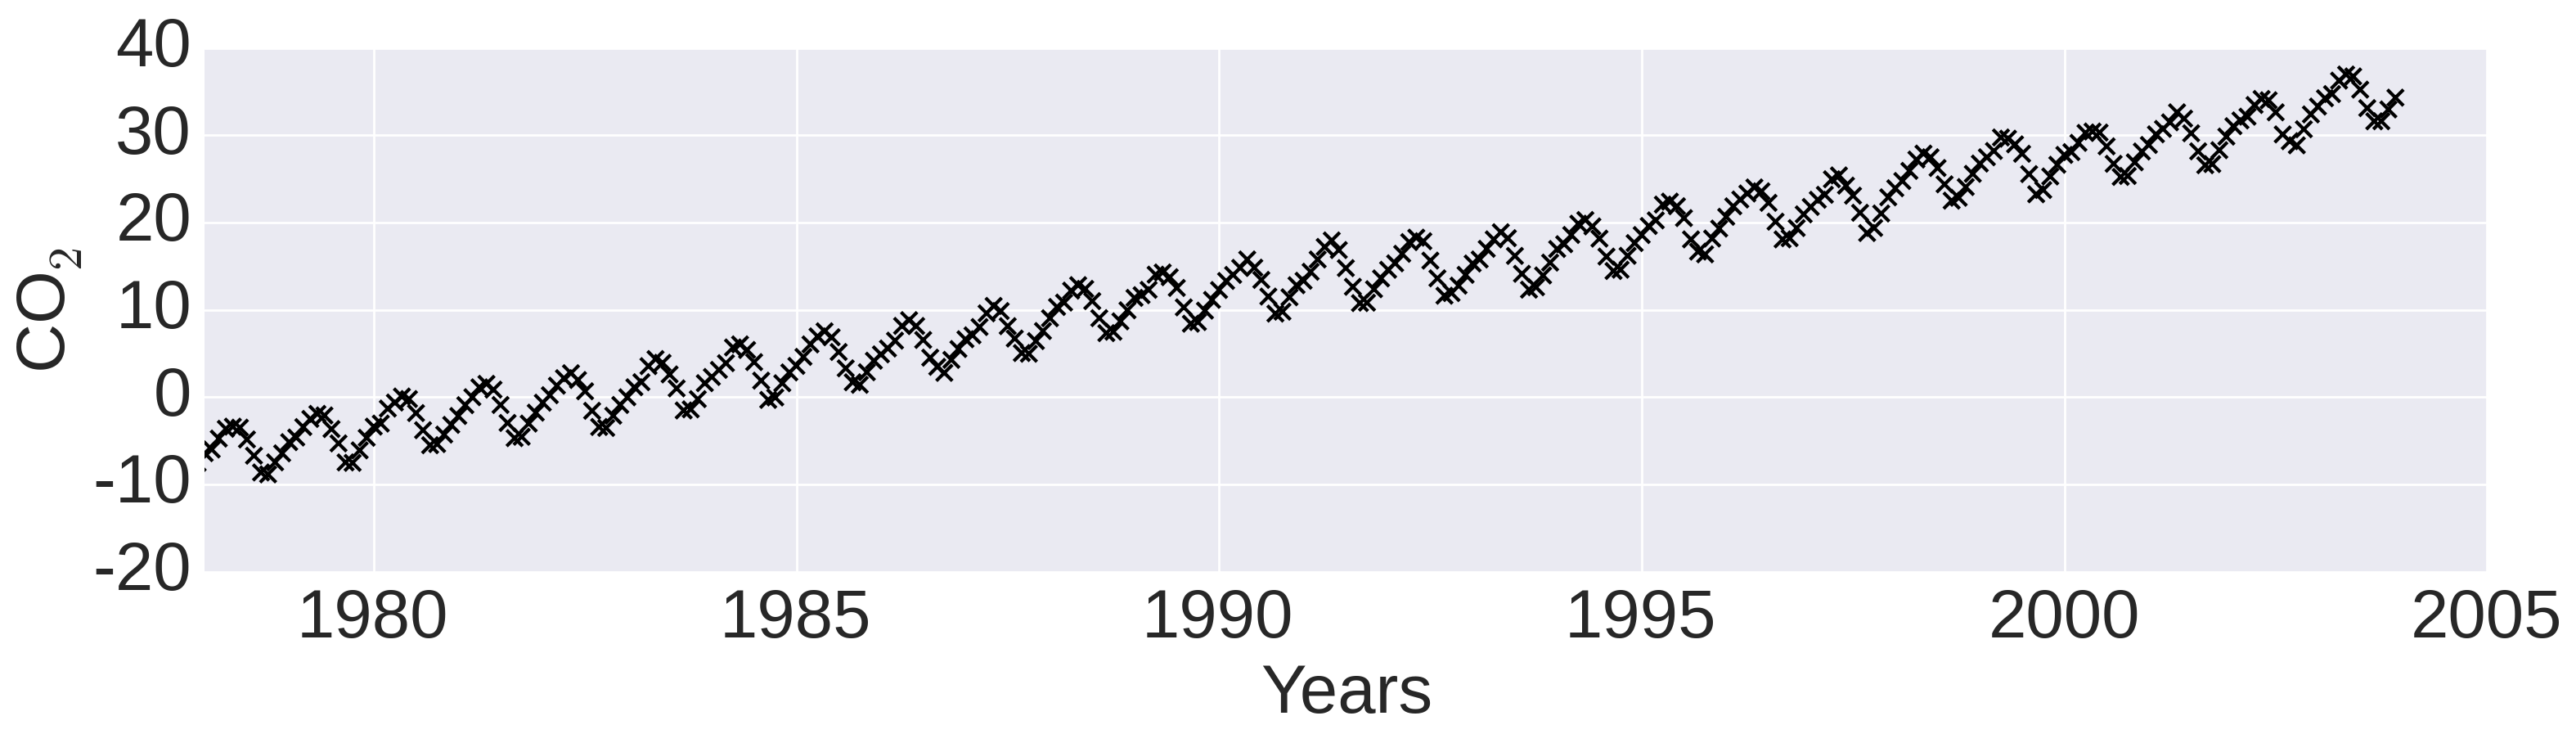
\includegraphics[width=0.7\textwidth]{figs/mauna_data.png}};
\node[below = 2.5cm of data] (post_param_helper) {};
\node[above = 1cm of post_param_helper] (post_param_helper_1) {};
\node[below = 1cm of post_param_helper] (post_param_helper_2) {};
\node[left = -3cm of post_param_helper] (post_param) {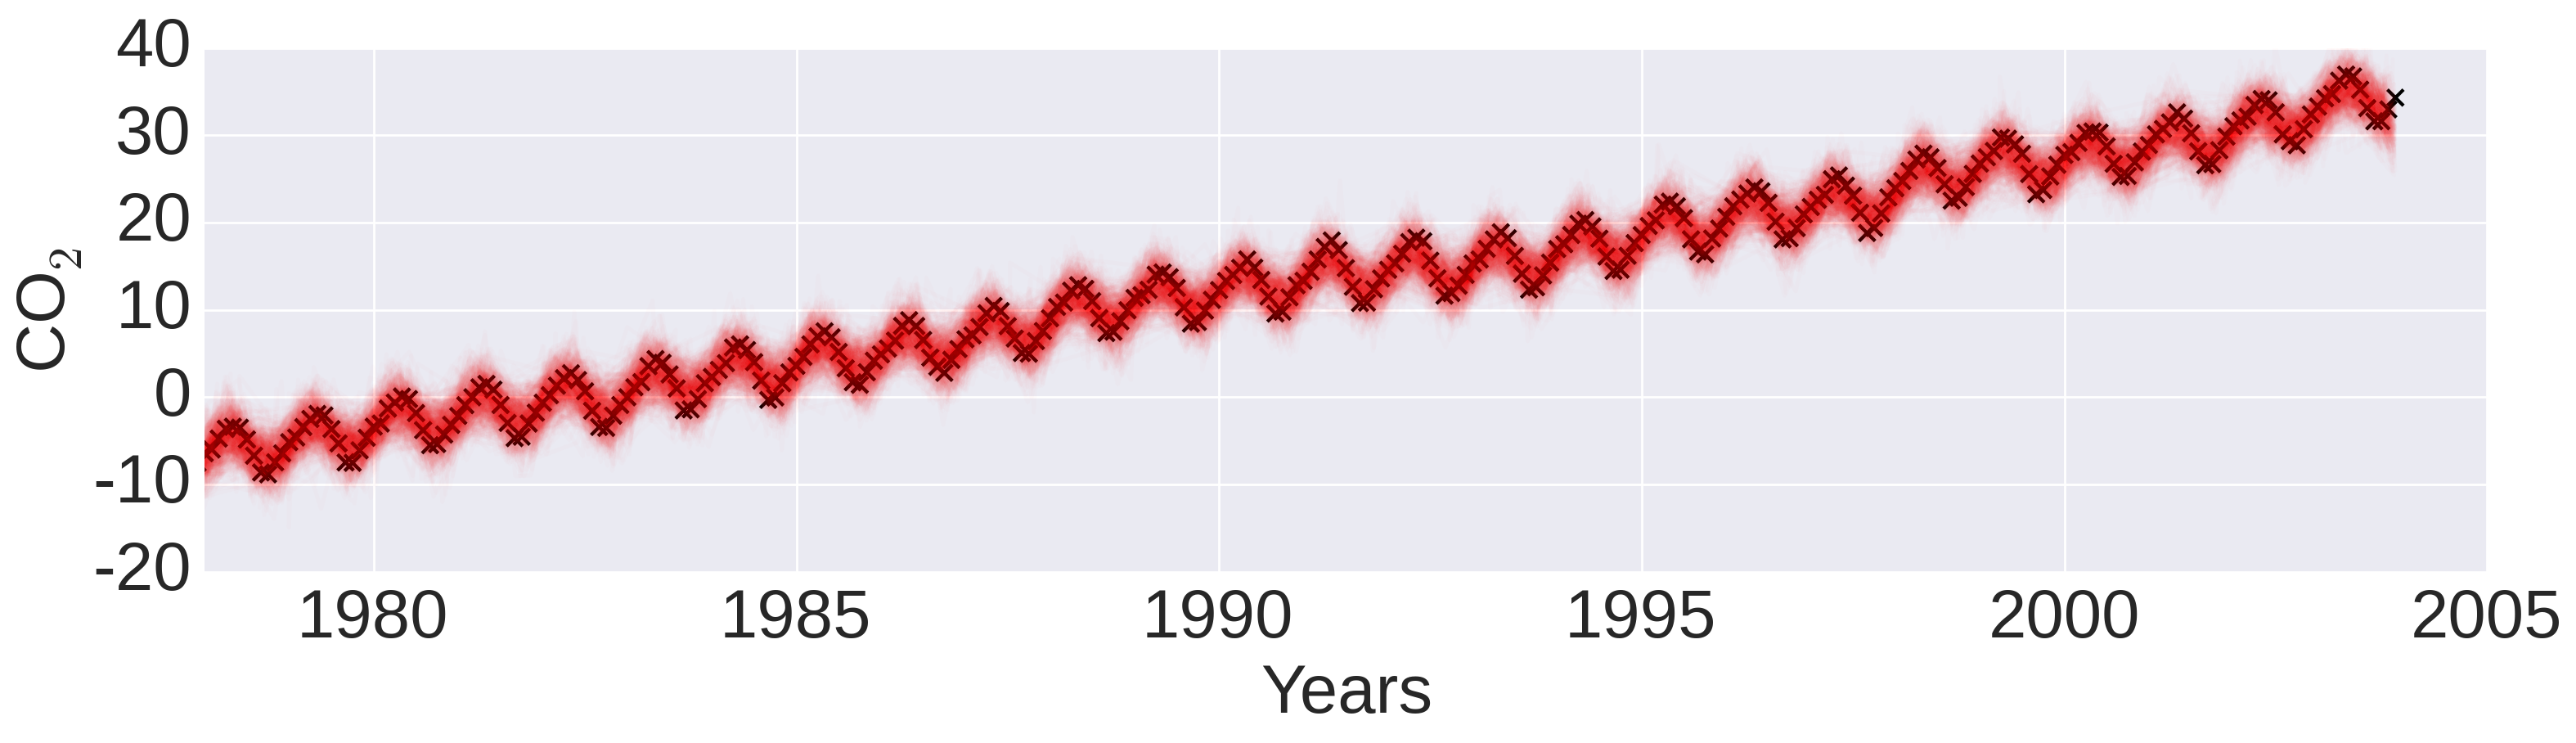
\includegraphics[width=0.6\textwidth]{figs/mauna_sample_1.png}};
\node[draw,rectangle,color=red,dashed,right = 4.5cm of post_param_helper,yshift=0.3cm] (zoom) {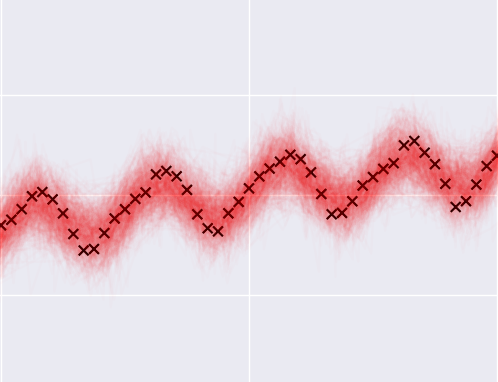
\includegraphics[width=0.2\textwidth]{figs/mauna_zoom.png}};
\node[draw,rectangle,color=red,dashed,left = 3.8cm of zoom, minimum width =
1.5cm, minimum height = 1.2cm,yshift=0.0cm] (zoom_in) {};
\node[below = 1.2cm of post_param_helper_2] (posterior) {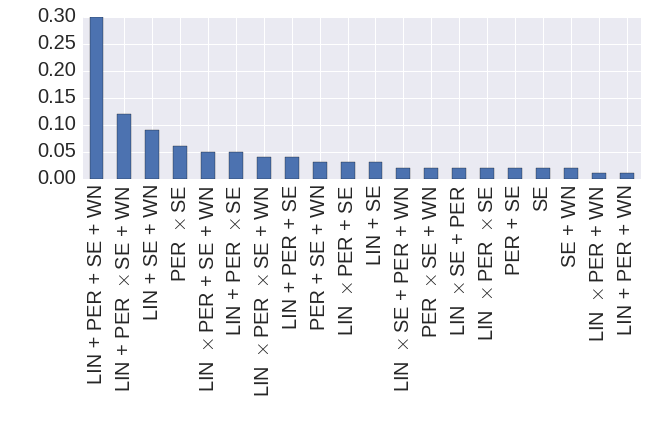
\includegraphics[width=0.6\textwidth]{figs/mauna_structure.png}};

\node[draw,rectangle,below = 1.2cm of posterior] (formula_param_1) {\color{black}\small
$\Ktheta= 2.7^2(x x^\prime) + 5.6^2 \exp \bigg( \frac{2 \sin^2 ( \pi (x - x^\prime)/3.7}{6.4^2} \bigg)
+ 0.4^2 \exp(-\frac{(x-x^\prime)^2}{2 \times 6.3^2}) +  1.9^2 \delta_{x,x^\prime} \label{eq:WN}$ };


\node[draw,rectangle,below = 1.2cm of formula_param_1,text width =
0.9\textwidth,minimum height = 1.5cm,font=\footnotesize] (paragraph){
The posterior peaks at a kernel structure with four additive components. Additive components hold globally, that is there are no higher level, qualitative aspects of the data that vary with the input space. The additive components are as follows: (i) a linearly increasing function or trend; (ii) a periodic function; (iii) a smooth function; and (iv) white noise.};







\node[draw, rectangle, left = -1.75cm of posterior,minimum width = 0.45cm, minimum height = 5.8cm,yshift=0.2cm] (mark_structure) {};
%\node[draw,very thick, rectangle, below = 1.1cm of data,minimum width = \textwidth, minimum height = 15cm] (posterior_frame) {};

%\node[left = 1.3cm of mark_structure] (paragraph_helper){};
\node[below =0.45cm of mark_structure,inner sep = 0pt,outer sep=0pt] (formula_helper) {};
\node[above =1.2cm of formula_param_1,inner sep = 0pt,outer sep=0pt] (formula_helper_2) {};

%\draw[-,dashed] (mark_structure.south) -- (formula_helper);
%\draw[-,dashed] (formula_helper) -- (formula_helper_2);
%\draw[->,dashed] (mark_structure) -- (paragraph_helper);
%\draw[->,dashed] (formula_helper_2) -- (formula);

\draw[->] (data) -- node[right]{\small $\hat \fbf \sim
\mathcal{N}(\hat{\bm{\mu}},\hat\Kbf)$} (post_param_helper_1);
\draw[->] (post_param_helper_2) -- node[right]{\small Posterior Structure} (posterior);
\draw[->] (formula_helper_2) -- node[right] {\small
$\bm{\theta}=\{2.7,5.6,3.7,6.4,0.4,6.3,1.9\}$} (formula_param_1);
\draw[-] (mark_structure) -- node[left, yshift=-0.3cm] {\small $\Ktheta$} (formula_helper);
\draw[-] (formula_helper) --(formula_helper_2);
\draw[->] (formula_param_1) -- node[right]{\small Qualitative Interpretation} (paragraph);

\draw[->,dashed,red] (zoom_in) --node[above]{\small\color{red}Zoom in:}
node[below]{\small\color{red}adequate error bars}(zoom);

%\draw[->,line width=1pt,double distance=2pt] (data) -- (post_param);
% starting from the bottom to aligm with caption 
\node[left=0.3cm of paragraph] (e){(e)}; 

\node[above=1.9cm of e] (d) {(d)}; 
\node[above=5.0cm of d] (c) {(c)}; 
\node[above=4.7cm of c] (b) {(b)}; 
\node[above=4.0cm of b] (a) {(a)}; 
\end{tikzpicture}
\addtolength\abovedisplayskip{1\baselineskip}%
\addtolength\belowdisplayskip{1\baselineskip}%



\caption{\footnotesize Structure Learning. Starting with raw data (a), we fit a \ac{GP}
(b) and compute the posterior distribution on structures (c). We take a sample
of the peak of this distribution ($\text{LIN}+\text{PER}+\text{SE}+\text{WN}$)
including its parameters and write it in functional form (d). We depict the
human readable interpretation (e). We used (d) to plot (b).}\label{fig:posterior}
\end{figure}
%%%%%%%%%%%%%%%%%%%%%%%%%%%%%%%%%%%%%%%%%%%%%%%%%%%%%%%%%%%%%%%%%%%%%%%%%%%%%%%%%
We illustrate results in Fig \ref{fig:posterior}. In Fig \ref{fig:posterior} (a) we depict the raw data. 
We see mean centered CO$_2$ measurements of the Mauna Loa Observatory, an atmospheric
baseline station on Mauna Loa, on the island of Hawaii. 
A description of the data set  can be found in  \citealp[][chapter 5]{rasmussen2006gaussian}.  
We use those raw data to compute a posterior on structure, parameters and \ac{GP}
samples.
The latter are shown in  Fig \ref{fig:posterior} (b)
where we zoom in to show how the posterior captures the error bars
adequately.
This posterior of the \ac{GP} is generated with a random sample from the parameters
of the peak of the distribution on structure (Fig \ref{fig:posterior} (c)).
We differentiate between a posterior distribution of kernel functions and  a
posterior distribution of
symbolic expressions describing different kernel structures. 
This allows us to compute the posterior of symbollically equivalent structures,
such as $\Struct(\klin + \kper)=\Struct(\kper + \klin)$. Both structures yield
and addition of a linear kernel and a periodic kernel, that is LIN + PER.
Therefore, we parse $k$ with $\Parse(k)$, we simplify an expression with $\Simplify(k)$ and
then compute $\Struct(k)$.
For the Mauna Loa Co$_2$ data, this distribution peaks at:
%%%%%%%%%%%%%%%%%%%%%%%%%%%%%%%%%%%%%%%%%%%%%%%%%%%%%%%%%%%%%%%%%%%%%%%%%%%%%%%%%
\begin{equation}
\Struct(\Ksrv=k)=\text{LIN} + \text{PER} + \text{SE} + \text{WN}.
\end{equation}
%%%%%%%%%%%%%%%%%%%%%%%%%%%%%%%%%%%%%%%%%%%%%%%%%%%%%%%%%%%%%%%%%%%%%%%%%%%%%%%%%
We write this kernel equation out in Fig \ref{fig:posterior} (d).
This kernel structure has a natural language interpretation that we spell out in
Fig \ref{fig:posterior} (e), explaining that 
the posterior peaks at a kernel structure with four additive components.
Each of which holds globally, that is there are no higher level, qualitative aspects
of the data that vary with the input space. The additive components for this result are as follows:
\begin{itemize}
\item a linearly increasing function or trend; 
\item a periodic function;
\item a smooth function; and
\item white noise.
\end{itemize}
 



Previous work on automated kernel discovery~\citep{duvenaud2013structure} illustrated the Mauna Loa data using an RQ kernel.
We resort to the white noise kernel instead of RQ (similar to \citep{lloyd2014automatic}).


%%%%%%%%%%%%%%%%%%%%%%%%%%%%%%%%%%%%%%%%%%%%%%%%%%%%%%%%%%%%%%%%%%%%%%%%%%%%%%%%%
%%%%%%%%%%%%%%%%%%%%%%%%%     Airline result   %%%%%%%%%%%%%%%%%%%%%%%%%%%%%%%%%%
%%%%%%%%%%%%%%%%%%%%%%%%%%%%%%%%%%%%%%%%%%%%%%%%%%%%%%%%%%%%%%%%%%%%%%%%%%%%%%%%
\myparagraph{Airline Data}
The second data set (Fig. \ref{fig:posterior_airline}) we depict results for is  the airline 
data set describing monthly totals of international airline passengers (\citealp{box2011time}, according to \citealp{duvenaud2013structure}). 
%%%%%%%%%%%%%%%%%%%%%%%%%%%%%%%%%%%%%%%%%%%%%%%%%%%%%%%%%%%%%%%%%%%%%%%%%%%%%%%%
\begin{figure}
\centering
 \addtolength\abovedisplayskip{-1\baselineskip}%
  \addtolength\belowdisplayskip{-1\baselineskip}%
  
\begin{tikzpicture}
\node (datatitle) {\small Raw Data};
\node[below = -0.25cm of datatitle](data) {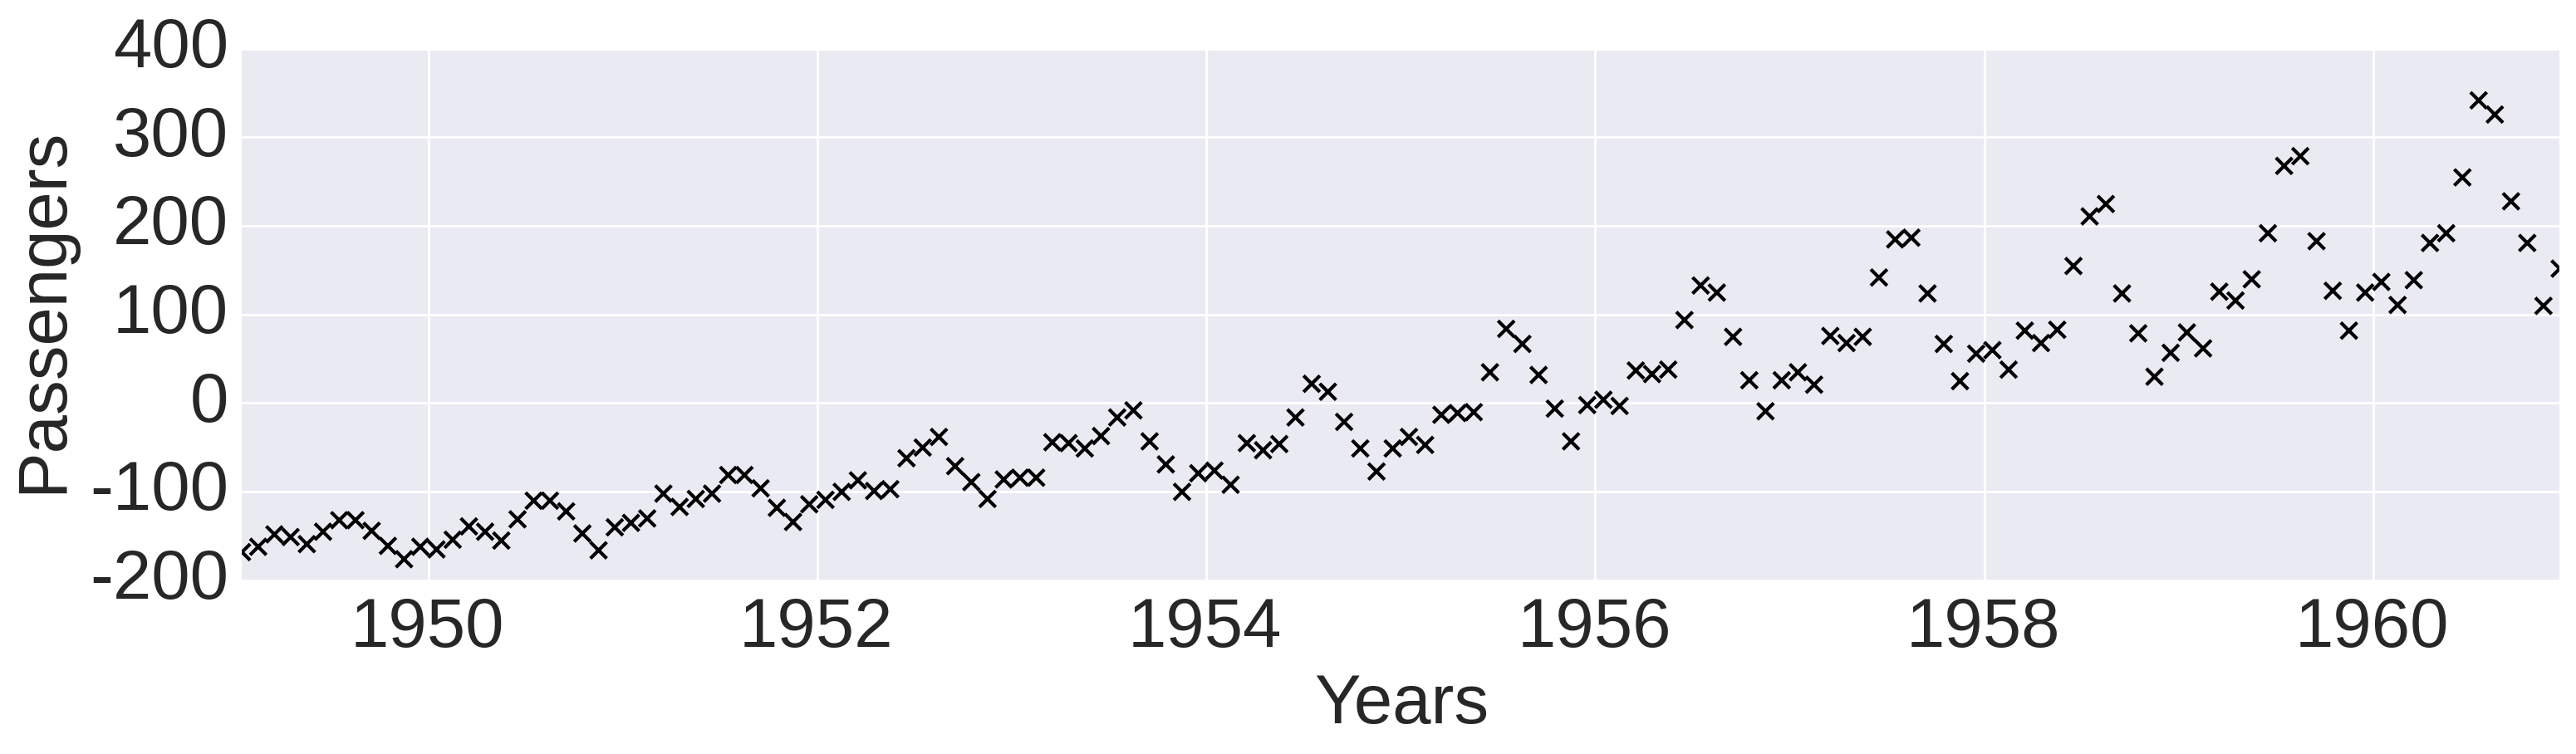
\includegraphics[width=0.65\textwidth]{figs/airline_data.png}};
\node[below= 1.2cm of data] (post_param) {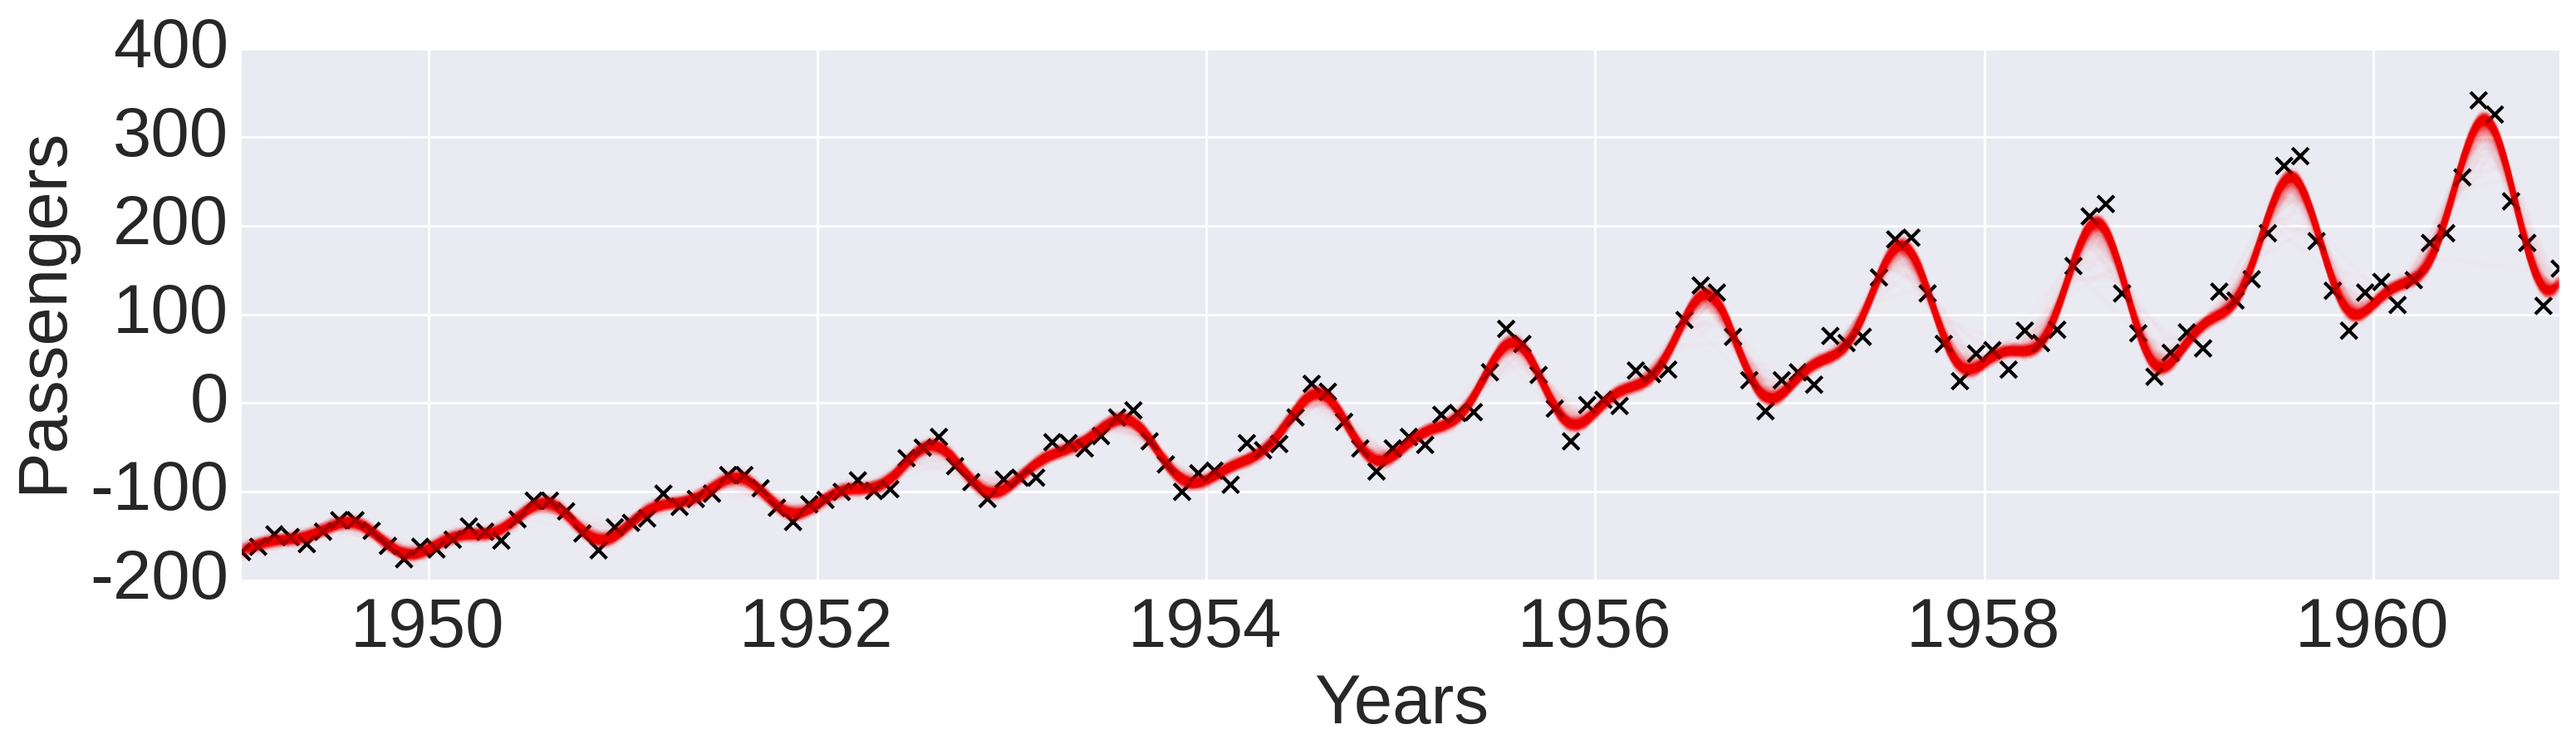
\includegraphics[width=0.65\textwidth]{figs/airline_sample_28.png}};


\node[below = 1.2cm of post_param] (posterior) {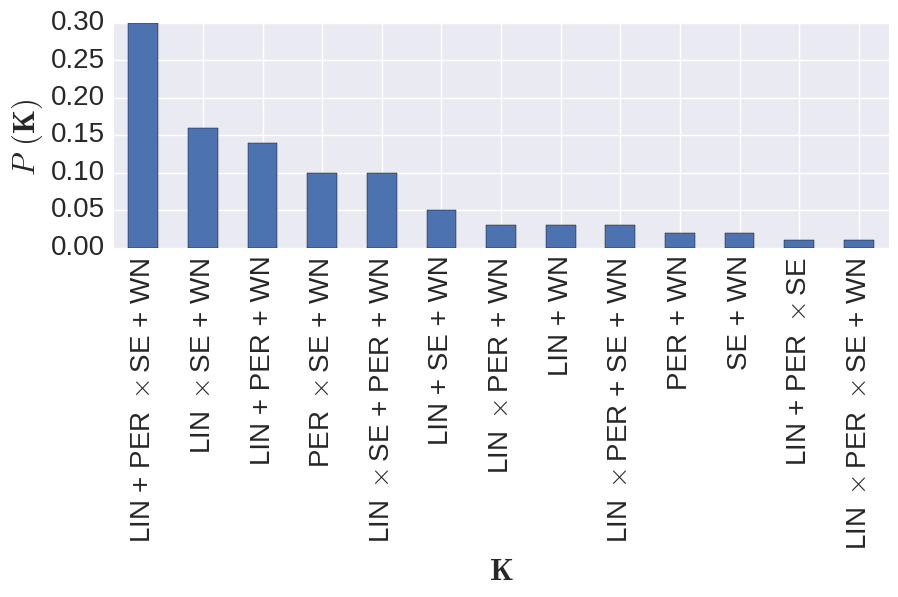
\includegraphics[width=0.55\textwidth]{figs/airline_structure.png}};
\node[below=-0.7cm of posterior,xshift=0.3cm] (xlabel) {\footnotesize
$\Ksrv$};
\node[left =-0.5cm of posterior,yshift=1.3cm] (ylabel) {\rotatebox{90}{\footnotesize
$P(\Ksrv \mid \xbf,\ybf, \thetabf )$}};
\node[draw,rectangle,below = 1.2cm of posterior] (formula_param_1) {\small\color{black}
$\ktheta= 7.47^2(x x^\prime) +
\Bigg(0.27^2 \exp(-\frac{(x-x^\prime)^2}{2 \times 4.63^2}) \times 
7.34^2 \exp \bigg( \frac{2 \sin^2 ( \pi (x - x^\prime)/4.4}{4.55^2} \bigg)\Bigg)
+ 2.93^2 \delta_{x,x^\prime} \label{eq:WN}$ };


\node[draw,rectangle,below = 1.2cm of formula_param_1,text width =0.9\textwidth,minimum height = 1.5cm, font=\footnotesize] (paragraph){ 
The posterior peaks at a kernel structure with three additive components.
Additive components hold globally, that is there are no higher level,
qualitative aspects of the data that vary with the input space. The additive
components are as follows: (i) a linearly increasing function or trend; (ii) an approximate periodic function; and (iv) white noise.};







\node[draw, rectangle, left = -1.7cm of posterior,minimum width = 0.45cm, minimum height = 5.2cm,yshift=0.2cm] (mark_structure) {};
%\node[draw,very thick, rectangle, below = 1.1cm of data,minimum width = \textwidth, minimum height = 15cm] (posterior_frame) {};

%\node[left = 1.3cm of mark_structure] (paragraph_helper){};
\node[below =0.45cm of mark_structure,inner sep = 0pt,outer sep=0pt] (formula_helper) {};
\node[above =1.2cm of formula_param_1,inner sep = 0pt,outer sep=0pt] (formula_helper_2) {};

%\draw[-,dashed] (mark_structure.south) -- (formula_helper);
%\draw[-,dashed] (formula_helper) -- (formula_helper_2);
%\draw[->,dashed] (mark_structure) -- (paragraph_helper);
%\draw[->,dashed] (formula_helper_2) -- (formula);

\draw[->] (data) -- node[right]{\small $\yprime \sim
\mathcal{N}(\mupost,\Kpost)$} (post_param_helper_1);
\draw[->] (post_param_helper_2) -- node[left]{\small }node[right]{\small Marginal on
Structure: $P(\Ksrv \mid \xbf,\ybf,\thetabf )$} (posterior);
\draw[->] (formula_helper_2) -- node[right] {\small
$\bm{\theta}=\{7.47,0.27,4.63,7.34,4.4,4.55,2.93\}$} (formula_param_1);
\draw[-] (mark_structure) -- node[left, yshift=-0.3cm] {\small $\ktheta$} (formula_helper);
\draw[-] (formula_helper) --(formula_helper_2);
\draw[->] (formula_param_1) -- node[right]{\small Qualitative Interpretation} (paragraph);


\node[left=0.3cm of paragraph] (e){(e)}; 

\node[above=1.9cm of e] (d) {(d)}; 
\node[above=5.0cm of d] (c) {(c)}; 
\node[above=4.7cm of c] (b) {(b)}; 
\node[above=4.0cm of b] (a) {(a)}; 
\end{tikzpicture}
\addtolength\abovedisplayskip{1\baselineskip}%
\addtolength\belowdisplayskip{1\baselineskip}%



\caption{\footnotesize Structure Learning. Starting with raw data (a), we fit a \ac{GP}
(b) and compute the posterior distribution on structures (c). We take a sample
of the peak of this distribution ($\text{LIN}+\text{PER} \times \text{SE}+\text{WN}$)
including its parameters and write it in functional form (d). We depict the
human readable interpretation (e). We used (d) to plot (b).}\label{fig:posterior_airline}
\end{figure}
%%%%%%%%%%%%%%%%%%%%%%%%%%%%%%%%%%%%%%%%%%%%%%%%%%%%%%%%%%%%%%%%%%%%%%%%%%%%%%%%

We illustrate results for this data set in Fig \ref{fig:posterior_airline}. In Fig \ref{fig:posterior_airline} (a) we depict the raw data. 
Again, the data is mean centered and we use it to 
compute a posterior on structure, parameters and \ac{GP}
samples.
The latter are shown in  Fig \ref{fig:posterior_airline} (b).
This posterior of the \ac{GP} is generated with a random sample from the parameters
of the peak of the distribution on structure (Fig \ref{fig:posterior_airline} (c)).
The posterior over symbolic kernel expressions peaks at:
%%%%%%%%%%%%%%%%%%%%%%%%%%%%%%%%%%%%%%%%%%%%%%%%%%%%%%%%%%%%%%%%%%%%%%%%%%%%%%%%%
\begin{equation}
\Struct(\Ksrv = k )=\text{LIN} +  \text{SE} \times \text{PER}+ \text{WN}.
\end{equation}
%%%%%%%%%%%%%%%%%%%%%%%%%%%%%%%%%%%%%%%%%%%%%%%%%%%%%%%%%%%%%%%%%%%%%%%%%%%%%%%%%
We write this Kernel equation out in Fig \ref{fig:posterior_airline} (d).
This kernel structure has a natural language interpretation that we spell out in
Fig \ref{fig:posterior_airline} (e), explaining that 
the posterior peaks at a kernel structure with three additive components.
Additive components hold globally, that is there are no higher level, qualitative aspects
of the data that vary with the input space.
The additive components are as follows: 
\begin{itemize}
\item a linearly increasing function or trend;
\item an approximate periodic function; and
\item  white noise.
\end{itemize}
Both datasets served as illustrations in the Automatic Statistician project.



%%%%%%%%%%%%%%%%%%%%%%%%%%%%%%%%%%%%%%%%%%%%%%%%%%%%%%%%%%%%%%%%%%%%%%%%%%%%%%%%%
%%%%%%%%%%%%%%%%%%%%%%%%% Queries for time series %%%%%%%%%%%%%%%%%%%%%%%%%%%%%%%
%%%%%%%%%%%%%%%%%%%%%%%%%%%%%%%%%%%%%%%%%%%%%%%%%%%%%%%%%%%%%%%%%%%%%%%%%%%%%%%%%
%%%%%%%%%%%%%%%%%%%%%%%%%%%%%%%%%%%%%%%%%%%%%%%%%%%%%%%%%%%%%%%%%%%%%%%%%%%%%%%%%
\myparagraph{Querying time series}
With our Bayesian approach to structure learning we can gain valuable insights
into time series data that were previously unavailable.
This is due to our ability to estimate posterior marginal probabilities over the kernel structure.
Over this marginal, we define boolean search operations that allow us to query the data
for the probability of certain structures to hold true globally.
%%%%%%%%%%%%%%%%%%%%%%%%%%%%%%%%%%%%%%%%%%%%%%%%%%%%%%%%%%%%%%%%%%%%%%%%%%%%%%%%%
\begin{align}
\label{eq:bool_present}
P(\Struct(\Ksrv=k) \mid \xbf,\ybf,\thetabf) =& \frac{1}{T}
\sum\limits_{t=1}^T \Cont(k,k^t)\\
&\text{where}\, \Cont(k,k^t) = \begin{cases}
  1, & \text{if } k \underset{global}{\in} k^t, \\
  0, & \text{otherwise}.
\end{cases} 
\end{align}
%%%%%%%%%%%%%%%%%%%%%%%%%%%%%%%%%%%%%%%%%%%%%%%%%%%%%%%%%%%%%%%%%%%%%%%%%%%%%%%%%
to ask whether it is true that a global structure $\Ksrv=k$ is present. $T$
is the number of all posterior samples for $\Ksrv$ and $k^t$ is one such
sample. $\underset{global}{\in} k^t$ reads as ``is one of $k^t$'s global
functional components".
We can now ask simple questions, for example:
\begin{quotation}
Is there white noise in the data?
\end{quotation}
To answer this question we set $\Struct(\Ksrv) = $WN in (\ref{eq:bool_present}). We write this in
shorthand as $\WNK$. Similarly, we write $\LINK$, $\PERK$ and $\SEK$. 
We can also formulate more sophisticated search operations using Boolean operators such as AND ($\land$) and OR ($\lor$).
The AND operator is defined as follows:
%%%%%%%%%%%%%%%%%%%%%%%%%%%%%%%%%%%%%%%%%%%%%%%%%%%%%%%%%%%%%%%%%%%%%%%%%%%%%%%%%
\[
P(\Struct(\Ksrv^a=k^a)\, \land\, \Struct(\Ksrv^b=k^b) \mid \xbf,\ybf, \thetabf)  = \frac{1}{N}
\sum\limits_{n=1}^N \Cont(k^a,k^t)\, \land \, \Cont(k^b,k^t)\;\;
\]
%%%%%%%%%%%%%%%%%%%%%%%%%%%%%%%%%%%%%%%%%%%%%%%%%%%%%%%%%%%%%%%%%%%%%%%%%%%%%%%%%
where
\[
\Cont(k^a,k^t) \land \Cont(k^b,k^t) = \begin{cases}
  1, & \text{if } k^a\, \text{and}\, k^b  \underset{global}{\in} k^t, \\
  0, & \text{otherwise}\end{cases}.
\]


%%%%%%%%%%%%%%%%%%%%%%%%%%%%%%%%%%%%%%%%%%%%%%%%%%%%%%%%%%%%%%%%%%%%%%%%%%%%%%%%%
\begin{figure}
\centering

% 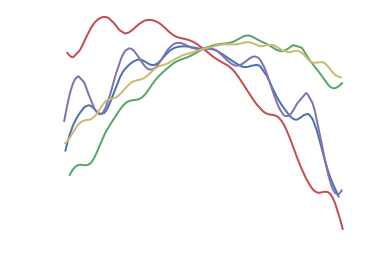
\includegraphics[width=.153\textwidth]{figs/gpSamples/main.png}
\begin{tikzpicture}


% level 1
\node (hyp) {\normalsize \color{blue} What is the probability of a trend, a recurring pattern {\bf and} noise in the data?};
\node[below = -0.2cm of hyp] (hyp_form) {$P\big((\text{LIN}\lor\text{LIN}\times\text{SE})\land
(\text{PER}\lor\text{PER}\times\text{SE}\lor\text{PER}\times\text{LIN})\land
(\text{WN}\lor\text{LIN}\times\text{WN})\big) = 0.36$};

%level 3
\node[below =.5cm of hyp_form , xshift=-3cm] (trend) {\color{blue} Is there a trend?};
\node[below = -0.2cm of trend] (trend_form) {$P(\text{LIN}\lor\text{LIN}\times\text{SE}) = 0.65$};
\node[below = -0.2cm of trend_form] (trend_png) {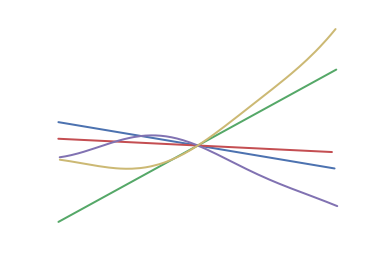
\includegraphics[width=.15\textwidth]{figs/gpSamples/trend.png}};

\node[below =.5cm of hyp_form, xshift=3cm] (noise) {\color{blue} Is there noise? };
\node[below = -0.2cm of noise] (noise_form) {$P(\text{WN}\lor\text{LIN}\times\text{WN}) = 0.75$};
\node[below = -0.2cm of noise_form] (noise_png) {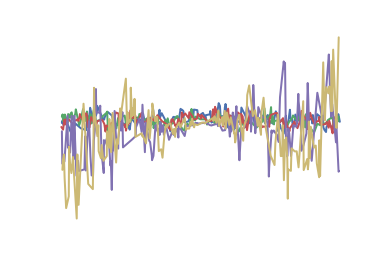
\includegraphics[width=.15\textwidth]{figs/gpSamples/noise.png}};

% level 4
\node[below =.5cm of trend_png , xshift=-2cm] (linear_trend) {\color{blue} A linear trend?};
\node[below = -0.2cm of linear_trend] (linear_trend_form) {$P(\text{LIN}) = 0.63$};
\node[below = -0.2cm of linear_trend_form] (linear_trend_png) {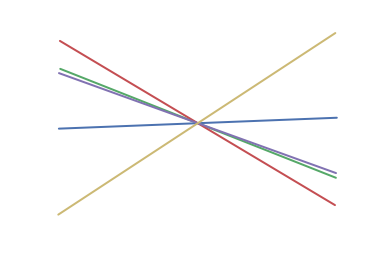
\includegraphics[width=.15\textwidth]{figs/gpSamples/lin.png}};

\node[below =.5cm of trend_png , xshift=1cm] (smooth_trend) {\color{blue} A smooth trend?};
\node[below = -0.2cm of smooth_trend] (smooth_trend_form) {$P(\text{LIN}\times\text{SE}) = 0.02$};
\node[below = -0.2cm of smooth_trend_form] (smooth_trend_png) {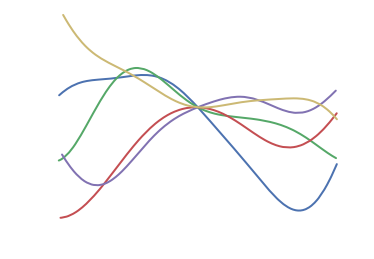
\includegraphics[width=.15\textwidth]{figs/gpSamples/selin.png}};

\node[below =.5cm of noise_png, xshift=-1cm] (het_noise) {\color{blue} Heteroskedastic noise? };
\node[below = -0.2cm of het_noise] (het_noise_form) {$P(\text{LIN}\times\text{WN}) = 0$};
\node[below = -0.2cm of het_noise_form] (het_noise_png) {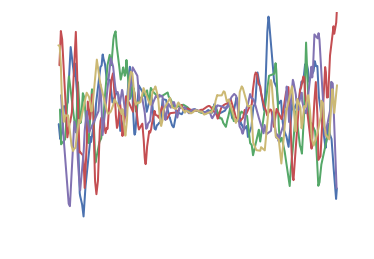
\includegraphics[width=.15\textwidth]{figs/gpSamples/linwn.png}};

\node[below =.5cm of noise_png, xshift=2cm] (white_noise) {\color{blue} White  noise? };
\node[below = -0.2cm of white_noise] (white_noise_form) {$P(\text{WN}) = 0.75$};
\node[below = -0.2cm of white_noise_form] (white_noise_png) {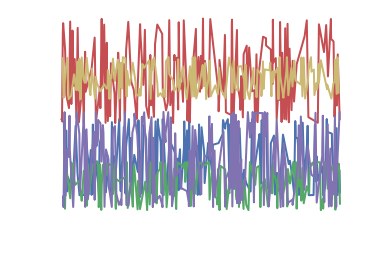
\includegraphics[width=.15\textwidth]{figs/gpSamples/wn.png}};

% level 5
\node[below =6.2cm of hyp_form] (recurring) {\color{blue} Is there repeating structure?};
\node[below = -0.2cm of recurring] (recurring_form) {$P(\text{PER}\lor\text{PER}\times\text{SE}\lor\text{PER}\times\text{LIN}) = 0.73$};
\node[below = -0.2cm of recurring_form] (recurring_png) {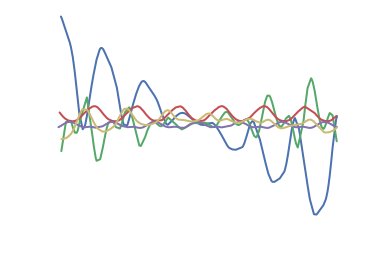
\includegraphics[width=.15\textwidth]{figs/gpSamples/recurring.png}};
%\draw[->,dashed] (barplot) -- (mcmc);

% level 6
\node[below =.5cm of recurring_png] (seper_form) {$\text{PER}\times\text{SE}=0.34$};
\node[below = -0.2cm of seper_form] (seper_png) {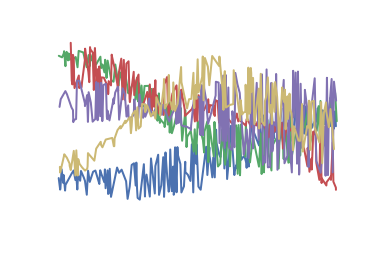
\includegraphics[width=.15\textwidth]{figs/gpSamples/seper.png}};

\node[below =.5cm of recurring_png, xshift=-3cm] (per_form) {$\text{PER}=0.32$};
\node[below = -0.2cm of per_form] (per_png) {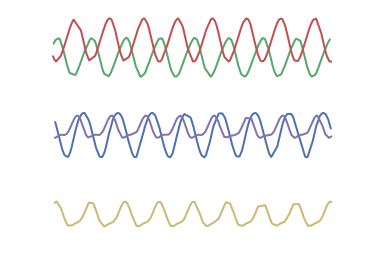
\includegraphics[width=.15\textwidth]{figs/gpSamples/per.png}};

\node[below =.5cm of recurring_png,xshift=3cm] (perlin_form) {$\text{PER}\times\text{LIN}=0.07$};
\node[below = -0.2cm of perlin_form] (seper_png) {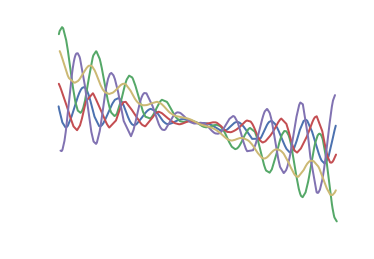
\includegraphics[width=.15\textwidth]{figs/gpSamples/perlin.png}};





\draw[->] (hyp_form) -- (trend);
\draw[->] (hyp_form) -- (noise);
\draw[->] (hyp_form) -- (recurring);


\draw[->] (noise_png) -- (het_noise);
\draw[->] (noise_png) -- (white_noise);

\draw[->] (trend_png) -- (linear_trend);
\draw[->] (trend_png) -- (smooth_trend);

\draw[->] (recurring_png) -- (per_form);
\draw[->] (recurring_png) -- (seper_form);
\draw[->] (recurring_png) -- (perlin_form);


\end{tikzpicture}



%  \multicolumn{3}{c}{$P(\text{PER}\lor\text{PER}\times\text{SE}\lor\text{PER}\times\text{LIN})$}

\caption{{\footnotesize \bf Querying structural motifs in in time series using posterior inference
over kernel structure.} The kernel structure serves as a way to formulate
natural language questions about the data (blue). The initial question of interest
(top) is a fairly
general one: ``What is the probability of a trend, a recurring
pattern and noise in the data?" Below the natural language version of this
question, the same question is formulated as an inference problem (black) over the
marginal probability on kernels with Boolean operators AND ($\land$) and OR ($\lor$). 
To gain  a deeper understanding of specific motifs in the time series more specific queries can
be written.
On the right, a query asks whether there is noise in the data (blue) by computing the disjunction of the marginal
of a global white noise kernel and a multiplication between a linear and a white
noise kernel (black). Samples from the predictive prior $\ybf_*$ of such kernels give an
indication of the qualitative aspects that a kernel structure implies (coloured curves below
the marginal). 
If the probability that there is noise in the data is high, it makes sense
to drill even deeper asking more detailed questions. With regards to noise, this
translates to querying whether or not the data supports the hypothesis that there is
heteroskedastic noise or white noise. Queries for motifs of repeating structure
are shown in the middle of the tree, queries related to trends on the left.}\label{fig:query}
\end{figure}
%%%%%%%%%%%%%%%%%%%%%%%%%%%%%%%%%%%%%%%%%%%%%%%%%%%%%%%%%%%%%%%%%%%%%%%%%%%%%%%%%
By estimating $P(\LINK \land \WNK \mid \xbf, \ybf, \thetabf)$ we can use this operator to ask questions such as 
\begin{quotation}
Is there a linear component AND a white noise in the data? 
\end{quotation}
Finally, we define the logical OR as
%%%%%%%%%%%%%%%%%%%%%%%%%%%%%%%%%%%%%%%%%%%%%%%%%%%%%%%%%%%%%%%%%%%%%%%%%%%%%%%%%
\begin{align*}
P(\Struct(\Ksrv^a)\, \lor\, \Struct(\Ksrv^b) \mid \xbf, \ybf, \thetabf)
=& P(\Struct(\Ksrv^a) \mid \xbf, \ybf, \thetabf) + P(\Struct(\Ksrv^b) \mid \xbf, \ybf, \thetabf)\\
 &- P(\Struct(\Ksrv^a) \land \Struct(\Ksrv^b) \mid \xbf, \ybf, \thetabf)
\end{align*}
%%%%%%%%%%%%%%%%%%%%%%%%%%%%%%%%%%%%%%%%%%%%%%%%%%%%%%%%%%%%%%%%%%%%%%%%%%%%%%%%%
where we drop $=k$ for readability. This allows us to ask questions about structures that are logically connected with OR, such as:
\begin{quotation}
Is there white noise or heteroskedastic noise?
\end{quotation}
by estimating $P(\LINK \times \WNK\;\;{\large\lor}\;\; \WNK \mid
\xbf, \ybf, \thetabf)$.
We know that noise can either be heteroskedastic or white,
and we also know due to simple manipulations using kernel algebra
that  $\text{LIN} \times \WN$ and $\text{WN}$ are the only possible ways to
construct noise with kernel composition. This allows us to generalize the 
question above to:
\begin{quotation}
Is there noise in the data? 
\end{quotation}
where we write the marginal posterior on qualitative structure for noise:
%%%%%%%%%%%%%%%%%%%%%%%%%%%%%%%%%%%%%%%%%%%%%%%%%%%%%%%%%%%%%%%%%%%%%%%%%%%%%%%%%
\begin{equation}
P\big(\Struct(\Ksrv)=\text{Noise} \mid \xbf, \ybf, \thetabf\big) = P(\LINK \times
\WNK\;\;{\large\lor}\;\; \WNK \mid \xbf, \ybf, \thetabf).
\end{equation}
%%%%%%%%%%%%%%%%%%%%%%%%%%%%%%%%%%%%%%%%%%%%%%%%%%%%%%%%%%%%%%%%%%%%%%%%%%%%%%%%%
From a methodological perspective, this allows us to start with general queries and 
subsequently formulate follow up queries that go into more detail.
For example, we could start with a general query, such as:
\begin{quotation}
What is the probability of a trend, a recurring pattern {\bf and} noise in the data?
\end{quotation}
and then follow up with more detailed questions (Fig \ref{fig:query}).

This way of querying data for their statistical implications is in stark contrast to what previous research in automatic kernel construction was able to provide.
We could view our approach as a time series search engine which allows us to test whether or not certain structures can be found
in an available time series.
Another way to view this approach is as a new language to interact with the world.
Real-world observations often come with time-stamps and in form
of continuous valued sensor measurements.  
We provide the toolbox to query such observations in a similar manner as
one would query a knowledge base in a logic programming language.






